\documentclass[11pt,letterpaper,titlepage]{article}
\usepackage[margin=2.54cm]{geometry}
\usepackage{graphicx}
\usepackage{float}

\title{60-475 Project One}
\author{David Mulatti \& Michael Necio}
\date{}

\begin{document}

	\maketitle
	\section{Implementation and Testing}
		\paragraph{}
			The implementation of the A-Priori, PCY, PCY multihash, and PCY
			multistage algorithms were made in a single C++ file, which iterates
			through various percentages of the \emph{retail.txt} data and
			outputs the runtime of the algorithms with various support
			thresholds. This data is then put into a .csv file, and graphed
			accordingly.

		\paragraph{}
			All experiments were run on a late 2011 MacBook Pro, running Mac OS
			10.12.3, with a 2.3GHz Intel i5 and 8GB of RAM.

	\section{Results With Provided Data}
		\paragraph{}
			In the graphs below, it is shown that A-Priori is the quickest
			algorithm for this data set. This is because the data set is fairly
			small, so the extra overhead of PCY does not result in a lower
			runtime. If we had a larger set of data, then it is likely that the
			payoff of PCY would be much more apparent.

		\paragraph{}
			PCY multihash and multistage are even slower, since it
			requires additional overhead to run, and the data set is not nearly
			large enough to see the payoff that these algorithms might provide.


		\begin{figure}[H]
			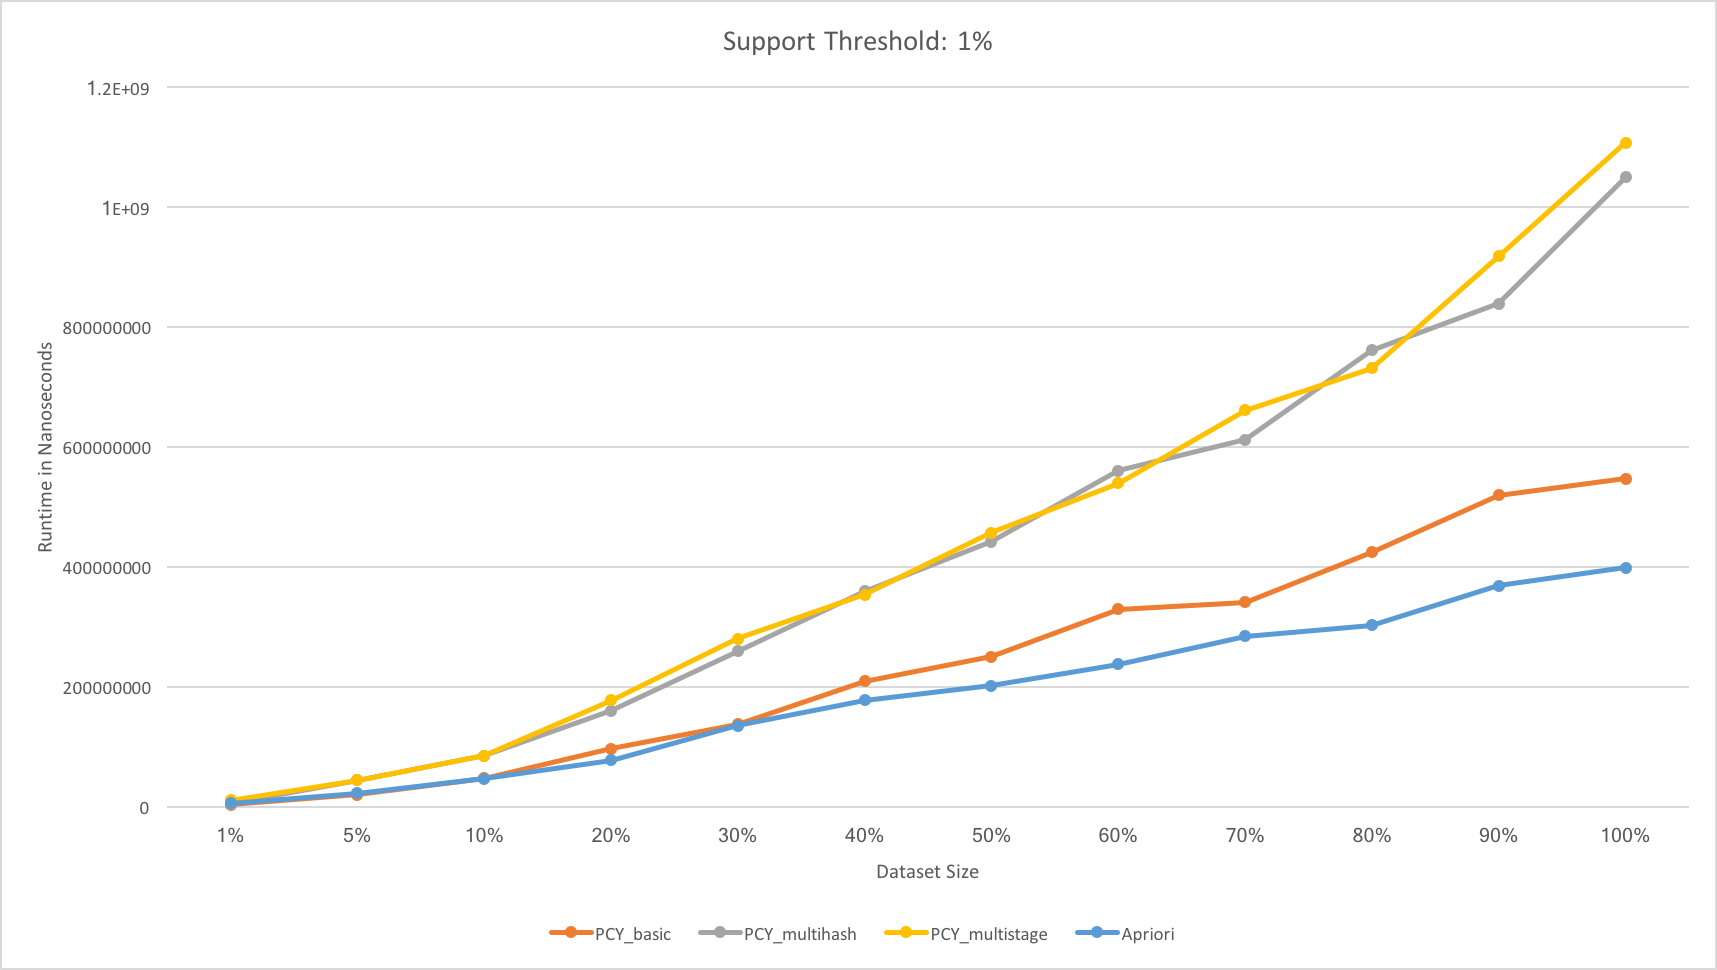
\includegraphics[width=\textwidth]{st1}
		\end{figure}

		\begin{figure}[H]
			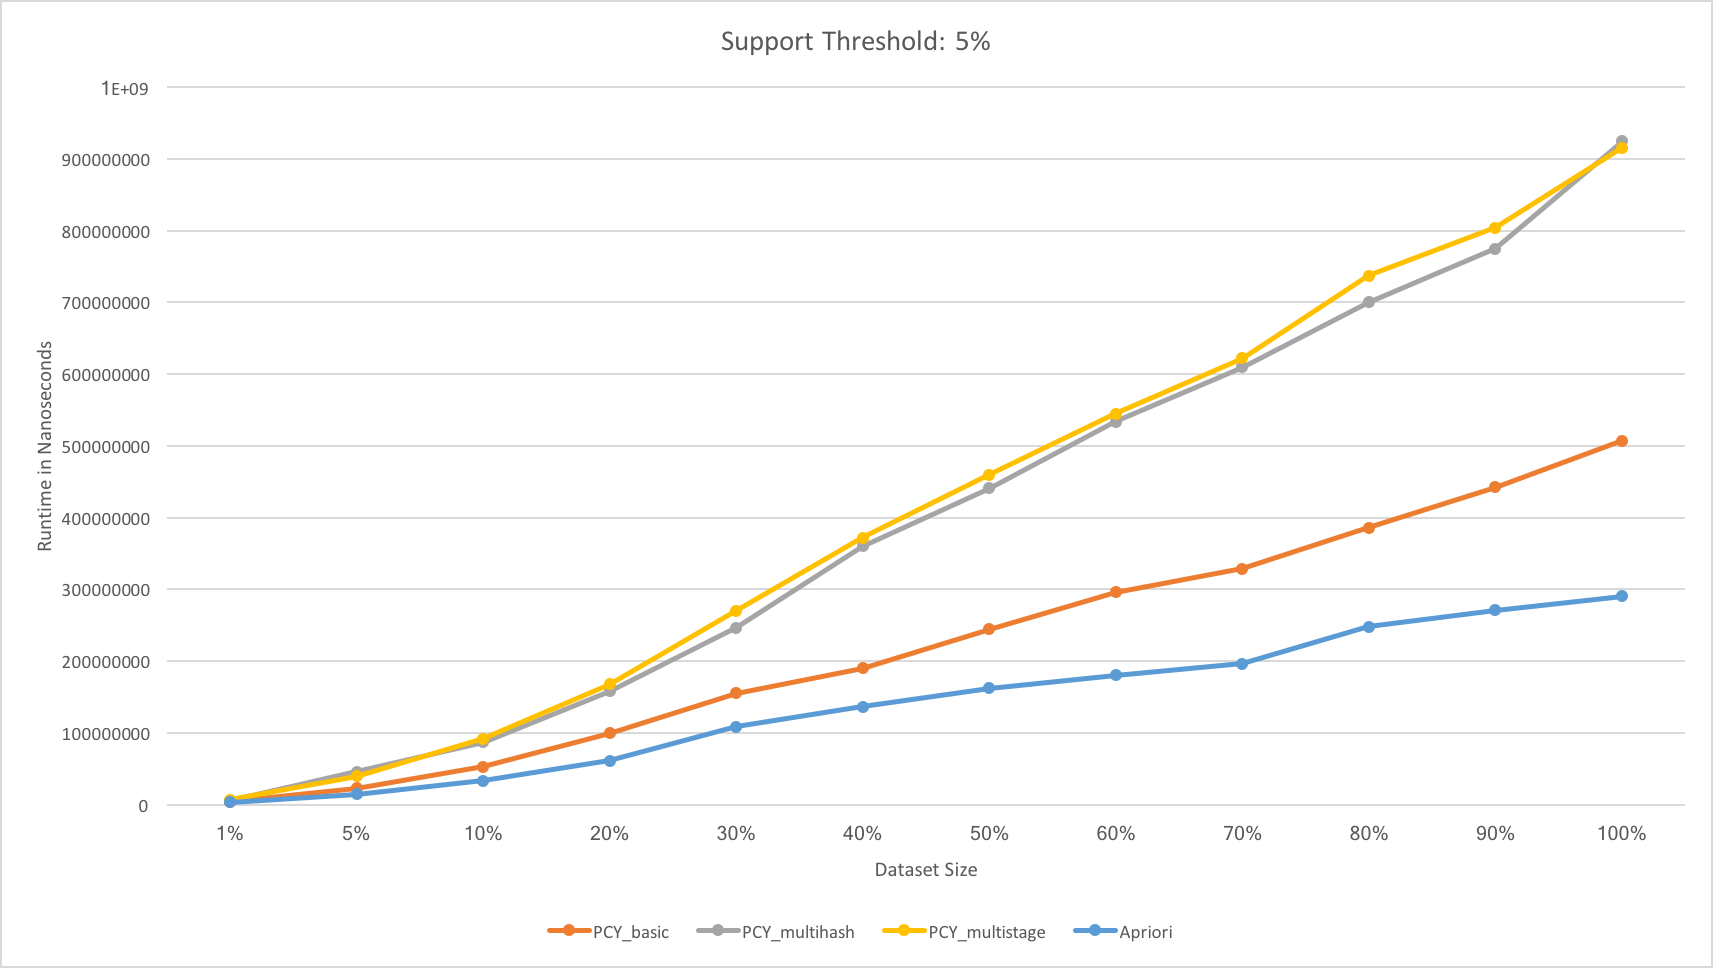
\includegraphics[width=\textwidth]{st5}
		\end{figure}

		\begin{figure}[H]
			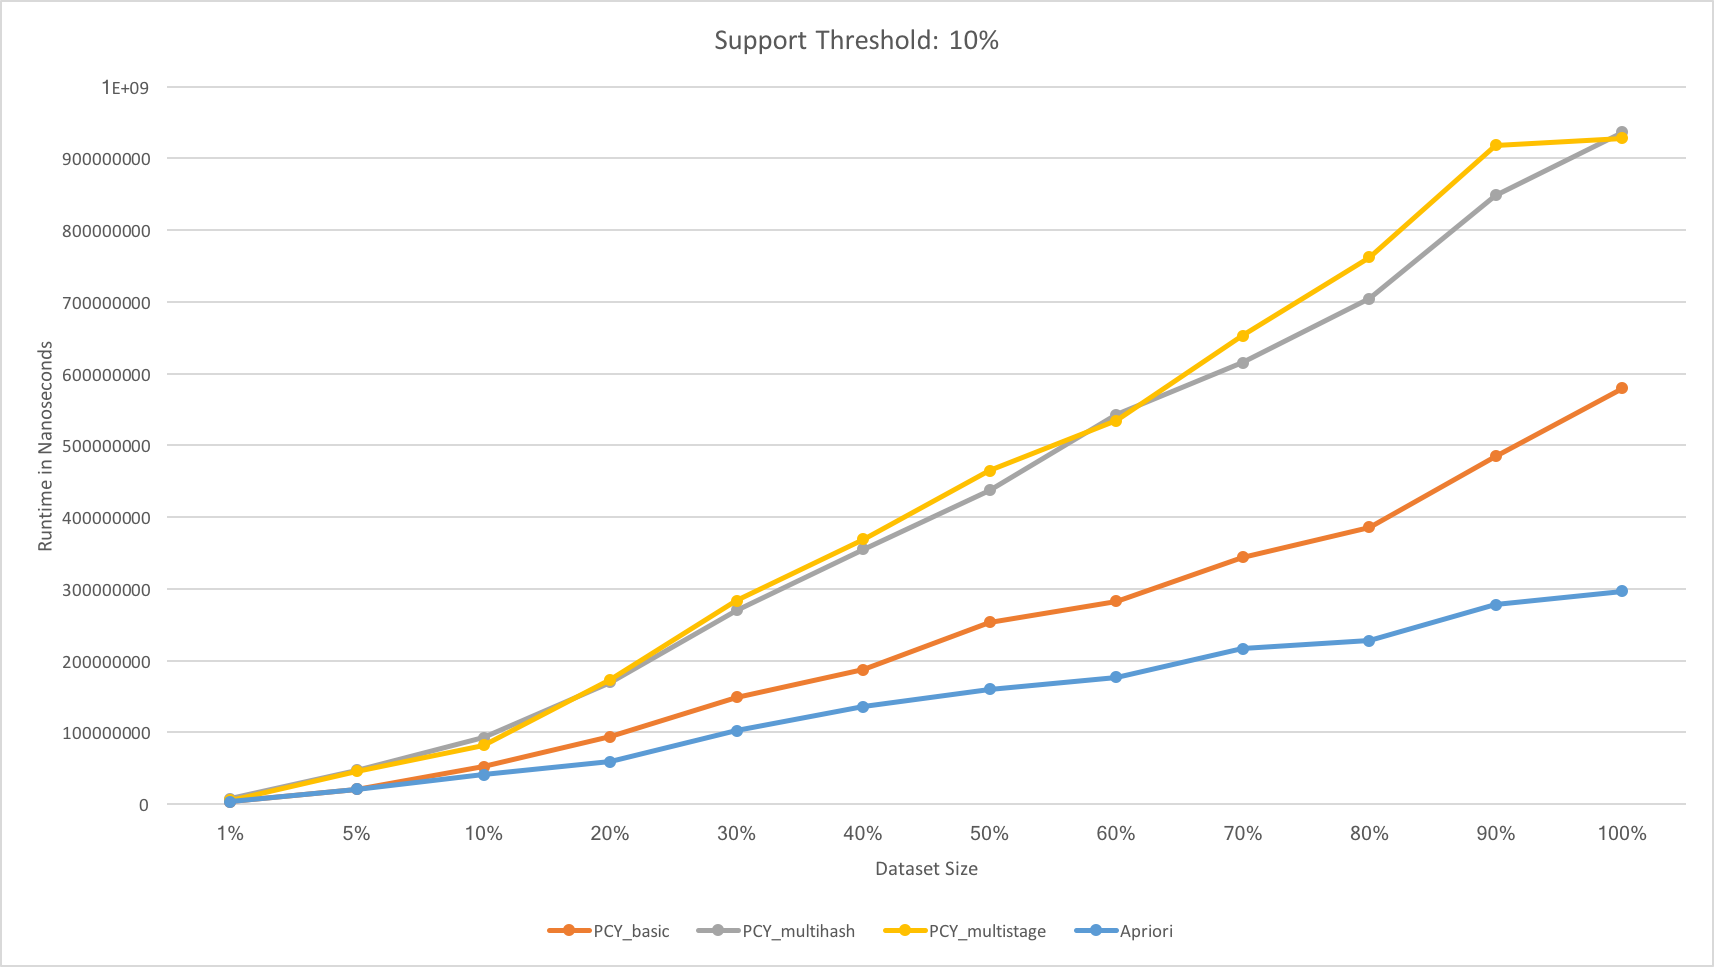
\includegraphics[width=\textwidth]{st10}
		\end{figure}

		\subsection{The Effects of Compiler Optimization}
		\paragraph{}
			An interesting observation that we noticed was that when we ran the
			program with clang's compiler optimizations enabled (set the -O3
			flag), PCY met or beat the performance of A-Priori with the same set
			of data. We suspect that this is due to the reduction of calls to
			the hashing function, as the compiler may have inserted its
			instructions inline.

		\begin{figure}[H]
			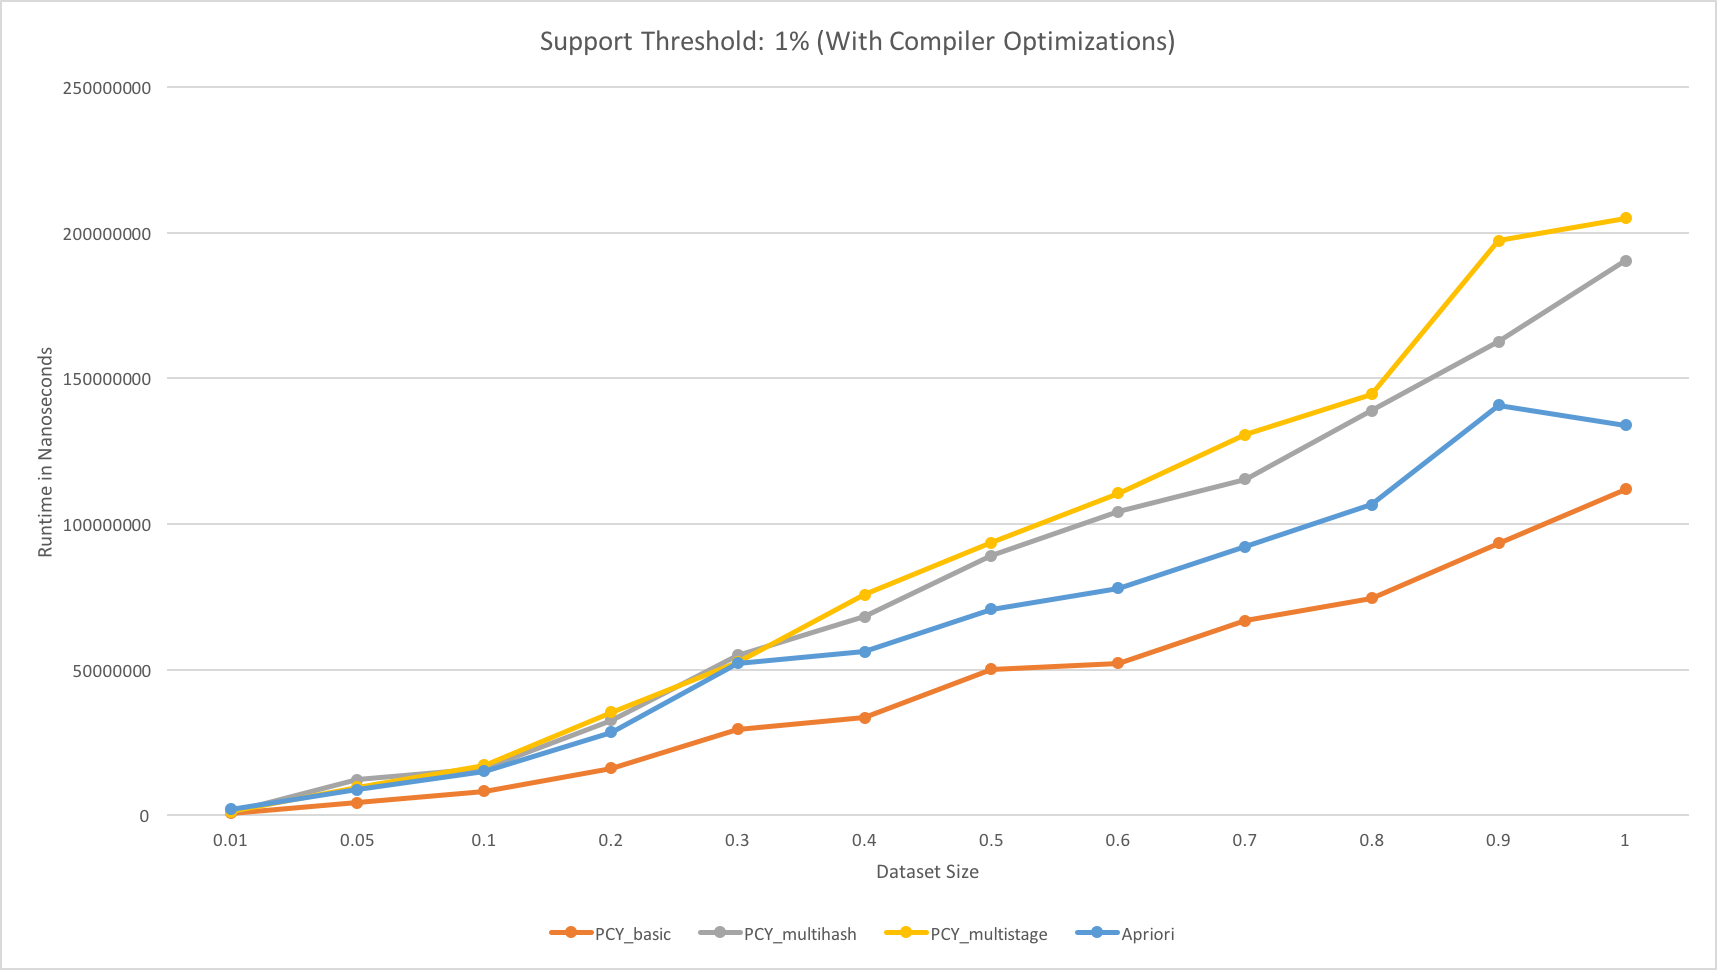
\includegraphics[width=\textwidth]{st1-opt}
		\end{figure}



	\section{Results with Large Randomized Data}
		\paragraph{}
			Since the provided dataset was not large enough to show off the true
			abilities of PCY, we wrote a python script that would generate a
			dataset with random baskets in the same format of \emph{retail.txt}.

		\paragraph{} We then fed a 100MB file into our C++ program, and got the
		following results:


		\begin{figure}[H]
			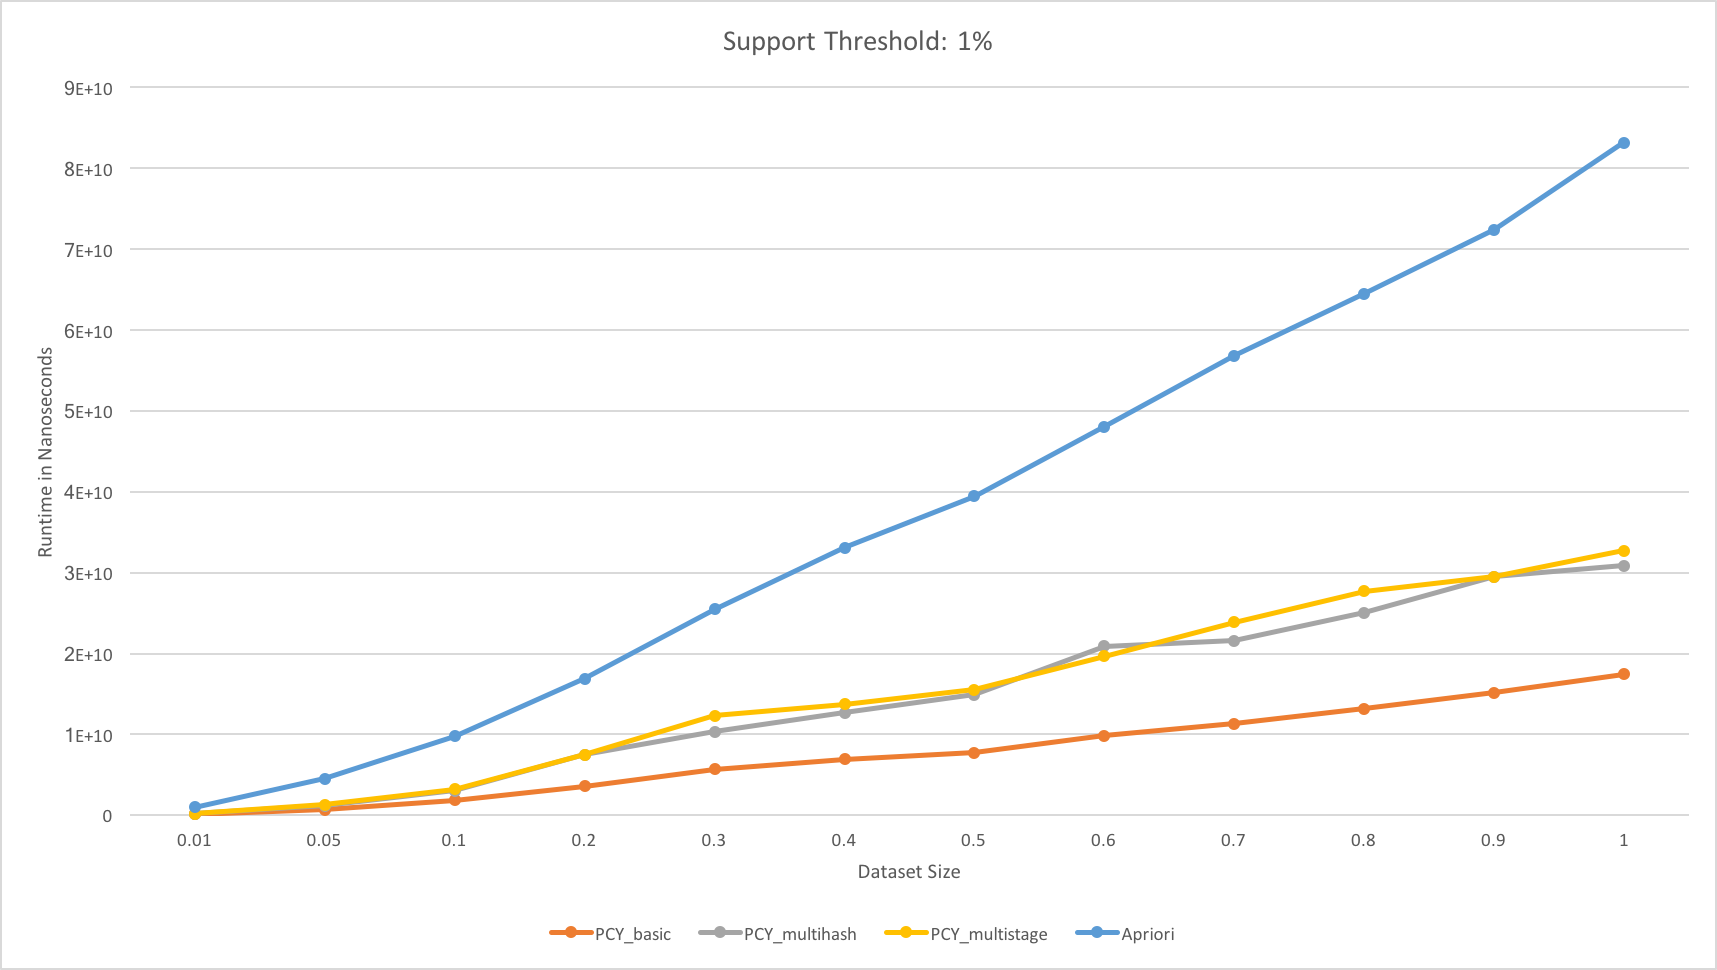
\includegraphics[width=\textwidth]{st1-big}
		\end{figure}

		\begin{figure}[H]
			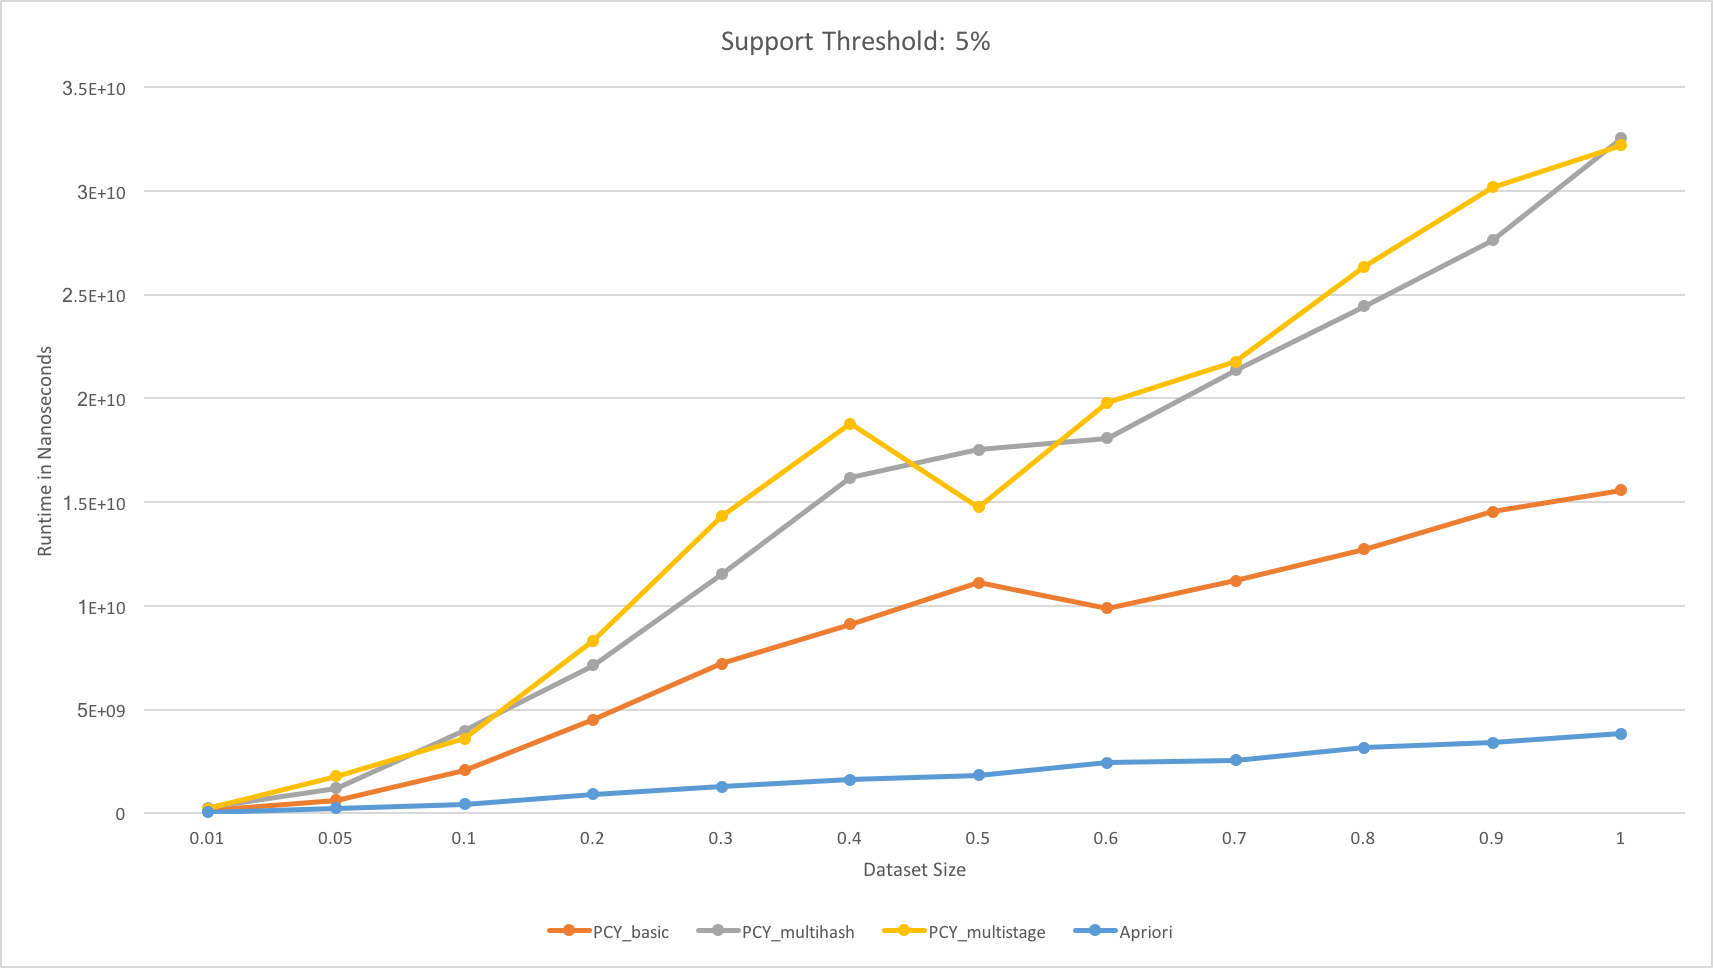
\includegraphics[width=\textwidth]{st5-big}
		\end{figure}

		\begin{figure}[H]
			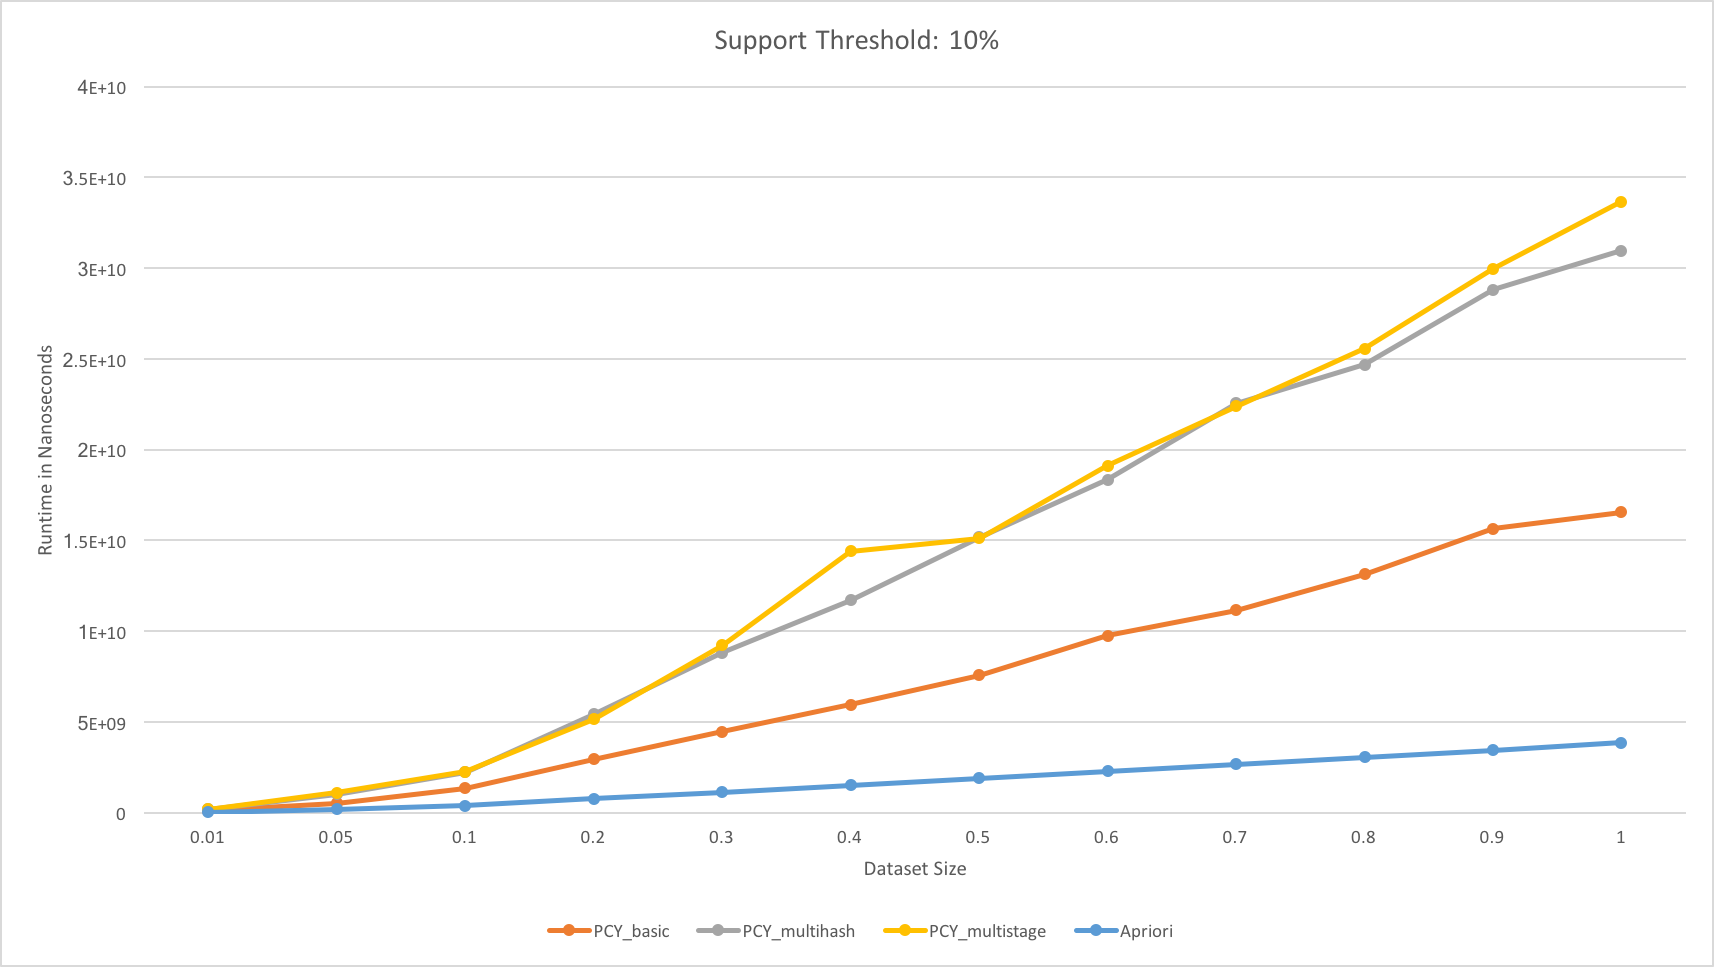
\includegraphics[width=\textwidth]{st10-big}
		\end{figure}

		\paragraph{}
			Here, we can see that when the support threshold is low, A-Priori is
			the slowest algorithm by far. However, when we raise the support
			threshold, the benefits of PCY disappear and A-Priori goes back to
			being the quickest.

	\section{Conclusion}
		\paragraph{}
			In conclusion, for the dataset provided it is best to use the
			A-Priori algorithm since it has the least amount of overhead and
			will run the quickest overall. It is only with large sets of data
			that the benefits of PCY are truly apparent.




\end{document}
